\chapter{Oxidation and Reduction of Alkenes}\label{ch:b2:alkene-redox}

Two-part epoxy glue comes in two tubes: one holds molecules ending in
\omterm{def:b2:alkene-redox:epoxide}{epoxide} rings, three-membered rings of two carbons and an oxygen; the other an
amine. Mixed, the strained rings open one after another and the paste sets
into a hard network. Alkenes are the raw material of such rings, of alcohols
placed where Markovnikov's rule would never put them, of diols with a chosen
geometry, and of the small fragments that once told chemists where a double
bond lay in a molecule. This chapter adds to the electrophilic additions of
the Year 1 volume the reactions that reduce or oxidise the double bond, and
the stereochemistry each one imposes.

\begin{recall}
The Year 1 volume: electrophilic additions, Markovnikov's rule, halonium ions,
syn and anti additions, hydration of alkenes, oxidation levels of carbon,
hydride donors, chemoselectivity, meso compounds and racemic mixtures,
stereospecific reactions. \Cref{ch:b2:catalytic-cycles}: the hydrogenation cycle of
Wilkinson's catalyst.
\end{recall}

\begin{omfigure}
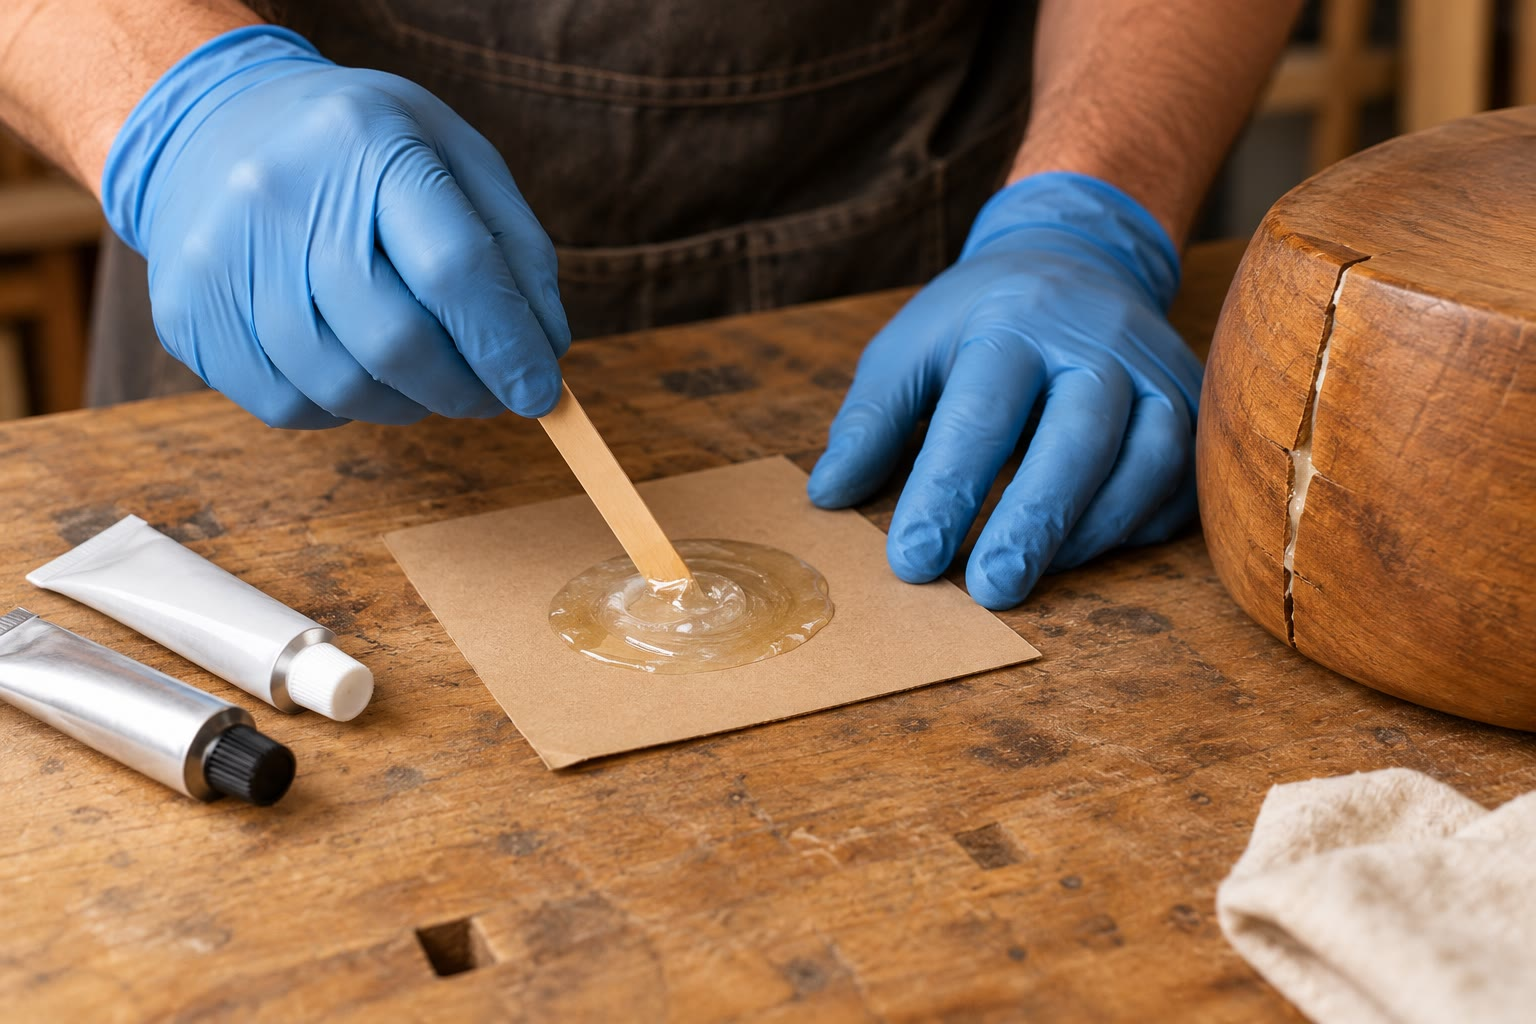
\includegraphics[width=0.6\linewidth]{images/book3/ai/b2-21-epoxy.jpg}

{\small Mixing a two-part epoxy glue: the resin, with \omterm{def:b2:alkene-redox:epoxide}{epoxide} groups, and the
hardener, an amine, react as soon as they meet; the rings open and link the molecules
into a solid network.}
\end{omfigure}

\section{Catalytic hydrogenation}

\begin{definition}[Catalytic hydrogenation]\label{def:b2:alkene-redox:hydrogenation}
A \emph{catalytic hydrogenation}\index{catalytic hydrogenation} adds dihydrogen across a
multiple bond in the presence of a catalyst: a finely divided metal (palladium on
carbon, platinum, nickel) in heterogeneous catalysis, or a soluble complex such as
Wilkinson's in homogeneous catalysis.
\end{definition}

On a metal surface, dihydrogen and the alkene are both held, the \ce{H-H} bond is broken
into surface hydrogen atoms, and these are transferred one after the other to the carbon
atoms of the alkene, which lies flat on the metal.

\begin{proposition}[Syn addition]\label{prop:b2:alkene-redox:syn-hydrogenation}
\omterm{def:b2:alkene-redox:hydrogenation}{Catalytic hydrogenation} delivers both hydrogen atoms to the same face of the double bond.
An alkyne hydrogenated over a poisoned palladium catalyst stops at the alkene, which is the
(\textit{Z}) isomer.
\end{proposition}

\begin{proof}[Argument]
The alkene is bound to the catalyst by one face, and both hydrogens come from the
catalyst, on that face: syn addition. With an alkyne, the two hydrogens added to the
triple bond are on the same side, cis to each other: the (\textit{Z})-alkene. A partly
deactivated catalyst (palladium on calcium carbonate with a lead salt and quinoline)
binds the alkyne much more strongly than the alkene formed, which leaves the surface
before a second addition.
\end{proof}

\section{Hydroboration--oxidation}

\begin{definition}[Hydroboration]\label{def:b2:alkene-redox:hydroboration}
A \emph{hydroboration}\index{hydroboration} adds a B--H bond of a borane across a
\ce{C=C} bond; followed by oxidation with alkaline hydrogen peroxide, it converts the
alkene into an alcohol whose hydroxyl group sits on the less substituted carbon: an
\emph{anti-Markovnikov orientation}\index{anti-Markovnikov orientation}.
\end{definition}

\begin{omfigure}
\setchemfig{atom sep=1.8em}
\schemestart[][west]
\chemfig{H_3C-[:30]CH=[:-30]CH_2}
\+ \chemfig{H-BH_2}
\arrow{->[syn addition]}
\chemfig{H_3C-[:30]CH_2-[:-30]CH_2-[:30]BH_2}
\arrow{->[\ce{H2O2}][\ce{HO-}]}
\chemfig{H_3C-[:30]CH_2-[:-30]CH_2-[:30]OH}
\schemestop
\par\vspace{6pt}

{\small Hydroboration--oxidation of propene. Borane adds in one step, boron to the
terminal carbon and hydrogen to the inner one, both on the same face; oxidation
replaces boron by \ce{OH} with retention of configuration. Propan-1-ol is formed, not the
propan-2-ol of acid-catalysed hydration.}
\end{omfigure}

\begin{proposition}[Orientation of hydroboration]\label{prop:b2:alkene-redox:hydroboration-regio}
Boron adds to the less substituted carbon of the double bond, and hydrogen to the more
substituted one; the addition is syn.
\end{proposition}

\begin{proof}[Argument]
Boron, with an empty p orbital, is the electrophile: in the four-centre transition state
(the two carbons, boron and hydrogen), the bond to boron forms a little ahead of the C--H bond, and a
partial positive charge develops on the other carbon, better carried by the more
substituted one; the bulky boron group also prefers the less hindered end. Both new bonds
form on one face, in a concerted step: syn.
\end{proof}

\begin{proposition}[Oxidation with retention]\label{prop:b2:alkene-redox:retention}
The oxidation of an alkylborane by alkaline hydrogen peroxide replaces each C--B bond by a
C--OH bond with retention of configuration at carbon.
\end{proposition}

\begin{proof}[Argument]
The hydroperoxide anion adds to boron; an alkyl group then migrates from boron to the
adjacent oxygen, with its pair of electrons, as hydroxide leaves; the carbon keeps its bonds
on the same side throughout. Hydrolysis of the B--O bond frees the alcohol.
\end{proof}

\section{Epoxides}

\begin{definition}[Epoxide]\label{def:b2:alkene-redox:epoxide}
An \emph{epoxide}\index{epoxide} (oxirane) is a cyclic ether with a three-membered ring of
two carbons and one oxygen. An \emph{epoxidation}\index{epoxidation} converts an alkene into
an epoxide, usually with a \emph{peroxy acid}\index{peroxy acid} \ce{RCO3H}, which transfers
one oxygen atom to the double bond.
\end{definition}

\begin{omfigure}
\setchemfig{atom sep=2em}
\schemestart
\chemfig{R-[:30]CH=[:-30]CH-[:30]R}
\+ \chemfig{Ar-C(=[2]O)-O-O-H}
\arrow{->}
\chemfig{[:-60]CH(-[:210]R)*3(-CH(-[:-30]R)-O-)}
\+ \chemfig{Ar-C(=[2]O)-OH}
\schemestop
\par\vspace{6pt}

{\small \omterm{def:b2:alkene-redox:epoxide}{Epoxidation} by a \omterm{def:b2:alkene-redox:epoxide}{peroxy acid} (Ar: for example a 3-chlorophenyl group). The terminal
oxygen of the \omterm{def:b2:alkene-redox:epoxide}{peroxy acid} is transferred to the double bond in one step, both C--O bonds
forming on the same face.}
\end{omfigure}

\begin{proposition}[Stereospecific epoxidation]\label{prop:b2:alkene-redox:epoxidation}
\omterm{def:b2:alkene-redox:epoxide}{Epoxidation} by a \omterm{def:b2:alkene-redox:epoxide}{peroxy acid} is stereospecific: a (\textit{Z})-alkene gives the cis \omterm{def:b2:alkene-redox:epoxide}{epoxide},
an (\textit{E})-alkene the trans \omterm{def:b2:alkene-redox:epoxide}{epoxide}.
\end{proposition}

\begin{proof}
The oxygen is transferred in one concerted step to one face of the double bond, which does
not rotate meanwhile: the relative positions of the substituents are kept.
\end{proof}

\begin{proposition}[Opening of epoxides]\label{prop:b2:alkene-redox:opening}
A nucleophile opens an \omterm{def:b2:alkene-redox:epoxide}{epoxide} by attack at one carbon from the face opposite to the oxygen
(anti opening, with inversion at that carbon). Under basic conditions, it attacks the less
hindered carbon; under acidic conditions, the more substituted one.
\end{proposition}

\begin{proof}[Argument]
The ring strain makes the C--O bonds easy to break. With a strong nucleophile and no acid,
the opening is a bimolecular substitution, and the least hindered carbon is reached most
easily. In acid the oxygen is protonated; the C--O bond to the more substituted carbon
stretches most, that carbon carrying the larger partial positive charge, and even a weak
nucleophile (water, an alcohol) attacks there --- still from the back, so still anti.
\end{proof}

\begin{omfigure}
\setchemfig{atom sep=2em}
\schemestart
\chemfig{[:-60]C(-[:210]H_3C)(-[:150]H_3C)*3(-CH_2-O-)}
\arrow{->[\ce{CH3O-}][\ce{CH3OH}]}[,1.4]
\chemfig{H_3C-C(-[2]CH_3)(-[6]OH)-CH_2-OCH_3}
\schemestop

\medskip
\schemestart
\chemfig{[:-60]C(-[:210]H_3C)(-[:150]H_3C)*3(-CH_2-O-)}
\arrow{->[\ce{CH3OH}][\ce{H+}]}[,1.4]
\chemfig{H_3C-C(-[2]CH_3)(-[6]OCH_3)-CH_2-OH}
\schemestop
\par\vspace{6pt}

{\small Opening of 2,2-dimethyloxirane by methanol. Top, with methoxide: attack at the
\ce{CH2}, the less hindered carbon. Bottom, in acid: attack at the more substituted carbon,
which carries most of the positive charge of the protonated \omterm{def:b2:alkene-redox:epoxide}{epoxide}.}
\end{omfigure}

\section{Dihydroxylation}

\begin{definition}[Dihydroxylation]\label{def:b2:alkene-redox:dihydroxylation}
A \emph{dihydroxylation}\index{dihydroxylation} converts an alkene into a 1,2-diol by adding
one \ce{OH} group to each carbon of the double bond.
\end{definition}

Osmium tetroxide, in catalytic amount with a reoxidant, and cold dilute permanganate add
both oxygens through a cyclic ester, on one face: a syn \omterm{def:b2:alkene-redox:dihydroxylation}{dihydroxylation}. \omterm{def:b2:alkene-redox:epoxide}{Epoxidation}
followed by opening with water in acid gives the anti diol.

\begin{proposition}[Syn and anti diols]\label{prop:b2:alkene-redox:diols}
From (\textit{Z})-but-2-ene, syn \omterm{def:b2:alkene-redox:dihydroxylation}{dihydroxylation} gives meso-butane-2,3-diol and the \omterm{def:b2:alkene-redox:epoxide}{epoxide}
route gives the racemic (2\textit{R},3\textit{R}) and (2\textit{S},3\textit{S}) diols; from
(\textit{E})-but-2-ene, the results are exchanged.
\end{proposition}

\begin{proof}
In (\textit{Z})-but-2-ene the two methyls are on the same side. Adding two \ce{OH} on one face
gives a diol in which, written in the eclipsed conformation of the former double bond, the
two \ce{OH} are on one side and the two methyls on the other: a mirror plane passes between
C2 and C3, the meso compound. The \omterm{def:b2:alkene-redox:epoxide}{epoxide} route puts the two \ce{OH} on opposite faces
(anti): the mirror plane is lost, and the attack at either carbon of the achiral \omterm{def:b2:alkene-redox:epoxide}{epoxide},
equally likely, gives the two enantiomers in equal amounts. For the (\textit{E})-alkene each
step changes the relation of the methyls, which exchanges the outcomes.
\end{proof}

\begin{omfigure}
\begin{tikzpicture}[font=\small]
  \begin{scope}
    \draw[thick] (0,0) -- (0,1.2);
    \draw[thick] (0,1.2) -- (-0.7,1.45); \draw[thick] (0,1.2) -- (0.7,1.45);
    \node[anchor=east] at (-0.7,1.45) {\ce{HO}}; \node[anchor=west] at (0.7,1.45) {\ce{CH3}};
    \draw[thick] (0,0) -- (-0.7,0.25); \draw[thick] (0,0) -- (0.7,0.25);
    \node[anchor=east] at (-0.7,0.25) {\ce{HO}}; \node[anchor=west] at (0.7,0.25) {\ce{CH3}};
    \node[anchor=south] at (0,1.25) {\scriptsize H};
    \node[anchor=north] at (0,-0.05) {\scriptsize H};
    \draw[densely dashed, omThm] (-1.6,0.6) -- (1.6,0.6);
    \node at (0,-1.0) {syn: meso};
  \end{scope}
  \begin{scope}[xshift=6.5cm]
    \draw[thick] (0,0) -- (0,1.2);
    \draw[thick] (0,1.2) -- (-0.7,1.45); \draw[thick] (0,1.2) -- (0.7,1.45);
    \node[anchor=east] at (-0.7,1.45) {\ce{HO}}; \node[anchor=west] at (0.7,1.45) {\ce{CH3}};
    \draw[thick] (0,0) -- (-0.7,0.25); \draw[thick] (0,0) -- (0.7,0.25);
    \node[anchor=east] at (-0.7,0.25) {\ce{H3C}}; \node[anchor=west] at (0.7,0.25) {\ce{OH}};
    \node[anchor=south] at (0,1.25) {\scriptsize H};
    \node[anchor=north] at (0,-0.05) {\scriptsize H};
    \node[align=center] at (0,-1.1) {anti: one enantiomer\\ (formed with its mirror image)};
  \end{scope}
\end{tikzpicture}

{\small The two butane-2,3-diols from (\textit{Z})-but-2-ene, schematic (vertical C2--C3
bond, the two groups of each carbon drawn left and right). Syn addition puts both
\ce{OH} on the same side: an internal mirror plane (dashed), the meso compound. Anti
addition puts them on opposite sides: a chiral diol, formed with its enantiomer.}
\end{omfigure}

\section{Oxidative cleavage}

\begin{definition}[Oxidative cleavage]\label{def:b2:alkene-redox:cleavage}
An \emph{oxidative cleavage}\index{oxidative cleavage} breaks both bonds of a \ce{C=C}
double bond and turns each carbon into a carbonyl or carboxyl group. In an
\emph{ozonolysis}\index{ozonolysis}, the alkene reacts with ozone and the intermediate
ozonide is decomposed in a second step, the work-up.
\end{definition}

\begin{proposition}[Products of ozonolysis]\label{prop:b2:alkene-redox:ozonolysis}
\omterm{def:b2:alkene-redox:cleavage}{Ozonolysis} splits each \ce{C=C} bond into two \ce{C=O} groups. With a reducing work-up
(zinc and acid, or dimethyl sulfide), a carbon bearing a hydrogen gives an aldehyde; with
an oxidising work-up (hydrogen peroxide), it gives a carboxylic acid. A carbon bearing two
carbon groups gives a ketone in both cases.
\end{proposition}

\begin{proof}[Argument]
Ozone adds to the double bond, the intermediate rearranges and the C--C bond breaks, giving
an ozonide in which each former alkene carbon is bound to two oxygens. The work-up reduces it
to two carbonyl compounds, or oxidises the aldehydes further. The intermediate steps are
admitted.
\end{proof}

\begin{omfigure}
\setchemfig{atom sep=2em}
\schemestart
\chemfig{H_3C-[:30]C(-[:90]CH_3)=[:-30]CH-[:30]CH_3}
\arrow{->[1. \ce{O3}][2. \ce{Zn}, \ce{H+}]}[,1.8]
\chemfig{H_3C-C(=[2]O)-CH_3}
\+
\chemfig{H-C(=[2]O)-CH_3}
\schemestop
\par\vspace{6pt}

{\small \omterm{def:b2:alkene-redox:cleavage}{Ozonolysis} of 2-methylbut-2-ene with a reducing work-up: propanone and
ethanal. Joining the two carbonyl carbons back by a double bond rebuilds the
alkene.}
\end{omfigure}

\begin{method}[Locating a double bond]\label{met:b2:alkene-redox:locate-double-bond}
\begin{enumerate}
  \item List the carbonyl fragments of the \omterm{def:b2:alkene-redox:cleavage}{ozonolysis} and count their carbons; they must add
        up to the alkene's.
  \item Each \ce{C=O} carbon was a doubly bonded carbon: join the fragments by replacing two
        \ce{C=O} by one \ce{C=C}.
  \item For a ring, one molecule with two carbonyl groups comes out; join its two ends.
  \item Check with the formula and the degree of unsaturation.
\end{enumerate}
\end{method}

Hot concentrated permanganate cleaves double bonds as well, giving acids and ketones; sodium
periodate cleaves 1,2-diols into two carbonyl compounds, a gentler route through the diol.

\begin{method}[Choosing a reagent for an alkene]\label{met:b2:alkene-redox:choose-reagent}
\begin{center}
\small
\renewcommand{\arraystretch}{1.15}
\begin{tabular}{lll}
target & reagent & stereochemistry, orientation \\ \hline
alkane & \ce{H2}, Pd/C & syn \\
Markovnikov alcohol & \ce{H2O}, acid & via a carbocation \\
anti-Markovnikov alcohol & \ce{BH3}, then \ce{H2O2}, \ce{HO-} & syn \\
\omterm{def:b2:alkene-redox:epoxide}{epoxide} & \omterm{def:b2:alkene-redox:epoxide}{peroxy acid} & stereospecific \\
syn diol & \ce{OsO4} (cat.) or cold \ce{MnO4-} & syn \\
anti diol & \omterm{def:b2:alkene-redox:epoxide}{peroxy acid}, then \ce{H2O}, acid & anti \\
two carbonyls & \ce{O3}, then \ce{Zn}/acid & cleavage \\
\end{tabular}
\end{center}
\end{method}

\begin{safety}{\ghs[5mm]{GHS02}\,\ghs[5mm]{GHS03}\,\ghs[5mm]{GHS05}\,\ghs[5mm]{GHS06}}
Osmium tetroxide is volatile and very toxic (it damages the eyes); it is used in catalytic
amount in solution, in a fume hood. \omterm{def:b2:alkene-redox:epoxide}{Peroxy acids} and hydrogen peroxide are oxidisers that
can decompose violently when heated or concentrated; borane solutions are flammable;
ozone is toxic and generated in a hood.
% ledger: ghs:OsO4, ghs:mCPBA, ghs:BH3-THF, ghs:O3, ghs:NaIO4
\end{safety}

\section{Exercises}

\begin{exercise}[$\star$]\label{exo:b2:alkene-redox:1}
Give the product of 1-methylcyclohexene with: \ce{H2}/Pd; \ce{H2O}/\ce{H+};
\ce{BH3} then \ce{H2O2}/\ce{HO-}; a \omterm{def:b2:alkene-redox:epoxide}{peroxy acid}; \ce{OsO4} (cat.); \ce{O3} then
\ce{Zn}/\ce{H+}.
\end{exercise}

\begin{exercise}[$\star$]\label{exo:b2:alkene-redox:2}
Which alcohol does hydroboration--oxidation give from 2-methylpropene? And acid-catalysed
hydration?
\end{exercise}

\begin{exercise}[$\star$]\label{exo:b2:alkene-redox:3}
Draw the \omterm{def:b2:alkene-redox:epoxide}{epoxide} formed from (\textit{E})-but-2-ene. Is it chiral?
\end{exercise}

\begin{exercise}[$\star$]\label{exo:b2:alkene-redox:4}
Give the products of the \omterm{def:b2:alkene-redox:cleavage}{ozonolysis} of hex-3-ene with a reducing work-up, then with an
oxidising work-up.
\end{exercise}

\begin{exercise}[$\star\star$]\label{exo:b2:alkene-redox:5}
Give the diols formed from (\textit{Z})-but-2-ene (a) with \ce{OsO4}; (b) with a \omterm{def:b2:alkene-redox:epoxide}{peroxy
acid} then aqueous acid. Which one is optically inactive because it is meso, and which
because it is racemic?
\end{exercise}

\begin{exercise}[$\star\star$]\label{exo:b2:alkene-redox:6}
2,2-Dimethyloxirane is opened by water in acid and by hydroxide. Do the two routes give the
same product? Explain.
\end{exercise}

\begin{exercise}[$\star\star$]\label{exo:b2:alkene-redox:7}
How would you prepare (\textit{Z})-hex-3-ene from hex-3-yne?
\end{exercise}

\begin{exercise}[$\star\star$]\label{exo:b2:alkene-redox:8}
An alkene \ce{C7H14} gives, by \omterm{def:b2:alkene-redox:cleavage}{ozonolysis} with a reducing work-up, propanone and butanal.
Give its structure.
\end{exercise}

\begin{exercise}[$\star\star$]\label{exo:b2:alkene-redox:9}
Propose a synthesis of hexan-1-ol from hex-1-ene, and say why acid-catalysed hydration
would fail.
\end{exercise}

\begin{exercise}[$\star\star\star$]\label{exo:b2:alkene-redox:10}
Limonene has a trisubstituted ring double bond and a disubstituted exocyclic one
(\ce{C(CH3)=CH2}). Which reacts first with one equivalent of a \omterm{def:b2:alkene-redox:epoxide}{peroxy acid}, and which with
one equivalent of a bulky borane? Explain.
\end{exercise}

\begin{exercise}[$\star\star\star$]\label{exo:b2:alkene-redox:11}
Prepare trans-cyclohexane-1,2-diol from cyclohexene, and cis-cyclohexane-1,2-diol.
\end{exercise}

\begin{exercise}[$\star\star\star$]\label{exo:b2:alkene-redox:12}
A compound \ce{C6H10} absorbs one equivalent of \ce{H2}. Its \omterm{def:b2:alkene-redox:cleavage}{ozonolysis} with a reducing
work-up gives a single product, hexanedial \ce{OHC-(CH2)4-CHO}. Identify it.
\end{exercise}

\section{Problem: Identifying a Terpene}

\begin{problem}[{Weekend problem --- the formula and unsaturation of limonene, its
hydrogenation, the fragments of its ozonolysis, and the selective reactions of its two
double bonds}]
\label{pb:b2:alkene-redox:1}
Limonene, the scent of orange peel, has the formula \ce{C10H16}. It is
1-methyl-4-(prop-1-en-2-yl)cyclohex-1-ene: a ring double bond bearing a methyl, and an
exocyclic \ce{C(CH3)=CH2} group on the opposite carbon of the ring. $R =
\qty{8.314}{J/(K.mol)}$; molar masses (\unit{g/mol}): C 12.011, H 1.008.
% ledger: aw:C, aw:H, const:R, ghs:limonene

\medskip
\noindent\textbf{Part I --- Formula and hydrogenation.}
\begin{enumerate}
  \item Compute the molar mass of limonene.
  \item Compute its degree of unsaturation.
  \item How many rings and how many double bonds does it have?
  \item Write its hydrogenation over palladium, product included.
  \item Compute the amount of dihydrogen absorbed by \qty{1.00}{g} of limonene.
  \item Compute its volume at \qty{25}{\degreeCelsius} and \qty{1.00}{bar}.
  \item Is the product chiral?
\end{enumerate}

\medskip
\noindent\textbf{Part II --- \omterm{def:b2:alkene-redox:cleavage}{Ozonolysis}.}
\begin{enumerate}[resume]
  \item Which fragments does \omterm{def:b2:alkene-redox:cleavage}{ozonolysis} with a reducing work-up give? (Count the carbons.)
  \item Why does the ring double bond give one molecule and not two?
  \item Which fragment is lost as a gas or volatile liquid?
  \item How would the products differ with an oxidising work-up?
  \item Show how the fragments locate the two double bonds.
  \item How many stereocentres does limonene have, and does the \omterm{def:b2:alkene-redox:cleavage}{ozonolysis} keep it?
\end{enumerate}

\medskip
\noindent\textbf{Part III --- \omterm{def:b2:alkene-redox:hydroboration}{Hydroboration}.}
\begin{enumerate}[resume]
  \item With one equivalent of a bulky borane, which double bond reacts? Why?
  \item Draw the product after oxidation.
  \item Is the new alcohol primary, secondary or tertiary?
  \item Why is the orientation called anti-Markovnikov?
  \item How many stereoisomers can form at the new stereocentre?
  \item Which reagent would instead put the \ce{OH} on the more substituted carbon of the
        same double bond?
\end{enumerate}

\medskip
\noindent\textbf{Part IV --- \omterm{def:b2:alkene-redox:epoxide}{Epoxidation}.}
\begin{enumerate}[resume]
  \item With one equivalent of a \omterm{def:b2:alkene-redox:epoxide}{peroxy acid}, which double bond reacts? Why?
  \item Draw the \omterm{def:b2:alkene-redox:epoxide}{epoxide}.
  \item Open it with water in acid: at which carbon does water attack?
  \item Draw the diol and give the relative orientation of its two \ce{OH}.
  \item How would you obtain the other diastereomer of this diol?
  \item State the volume of dihydrogen absorbed by \qty{1.00}{g} of limonene at
        \qty{25}{\degreeCelsius} and \qty{1}{bar}.
\end{enumerate}
\end{problem}
